
\documentclass[11pt,a4j]{jreport}

\usepackage{comment}
\usepackage{float}
\usepackage{color}
\usepackage{multicol}
\usepackage[dvipdfmx]{pict2e}
\usepackage{wrapfig}
\usepackage{graphicx}
\usepackage{bm}
\usepackage{url}
\usepackage{underscore}
\usepackage{colortbl}
\usepackage{tabularx}
\usepackage{fancyhdr}
\usepackage{ulem}
\usepackage{cite}
\usepackage{amsmath,amssymb,amsfonts}
\usepackage{algorithmic}
\usepackage{textcomp}
\usepackage{xcolor}
\usepackage[ipaex]{pxchfon}
\usepackage{booktabs}
\usepackage{multirow}
\usepackage{ulem}

\usepackage[top=30truemm,bottom=30truemm,left=25truemm,right=25truemm]{geometry}

\begin{document}

\thispagestyle{empty}
\begin{center}

\vspace{20mm}
{\Large\noindent 2024年度 卒業論文}\\
\vspace{40mm}
{\huge\noindent\textbf{警備員ロボットの抑止力向上のための}}\\
\medskip
{\huge\noindent\textbf{オペレータ支援システムの開発}}\\
\vspace{\baselineskip}
\vspace{40mm}

{\Large\noindent
2024年1月31日\\
\vspace{\baselineskip}
指導教員 神田  崇行\\
\vspace{\baselineskip}
京都大学\\
社会情報学研究科\\
\vspace{\baselineskip}
1029323422 天野岳洋\\
}
\vspace{40mm}

\end{center}

\thispagestyle{empty}
\clearpage

%=====================================================================================
\renewcommand{\abstractname}{要旨}

\begin{abstract}
アバターロボットが普及し、アバターを介して遠隔地から勤務することが新たな働き方として認められつつある。
しかし、特に警備員のような仕事を行う際には、たかがロボットと侮られることが多く、抑止力が低下するという問題がある。
そこで本論文では、注意時に引き起こされる認知的不協和と、その解消方法に注目することによって、より効果的な注意文言を作成し、それらをオペレータに
提示することで、抑止力を向上させることを目的としたオペレータ支援システムの開発を行った。

具体的には、注意時の移動操作を簡単にすることによって、
オペレータがより対話に集中できるようにすることに加えて、認知的不協和理論に基づいて、生じた不快感の解消法
に応じた注意文言を提案することによって、抑止力を高めることができるようになる。
また、この支援システムを用いることで、
操作に不慣れなオペレータであっても、より効果的にロボットを操作することができるようになるため、警備員の仕事を全うすることが容易になると考えられる。
\end{abstract}

%=====================================================================================

% 目次の表示
\tableofcontents

%=====================================================================================
\pagestyle{fancy}
\lhead{\rightmark}
\renewcommand{\chaptermark}[1]{\markboth{第\ \normalfont\thechapter\ 章~~#1}{}}
%=====================================================================================

\chapter{はじめに} %章

\section{研究背景} %1.1
\subsection{アバターロボットとは} %1.1.1
アバターロボットとは、人間が遠隔地に存在するロボットを操作することで、遠隔地に存在する人間の代理として行動するロボットである。アバターロボットは、リモートワークを可能にする。リモートワークは、働く場所を問わないことや
他の人間と直接接する機会が少ないことなどから、働きやすさの面やパンデミック時において、通常の働き方よりも有利である。またリモートワークは組織、従業員両者にとって利点があることがわかっている\cite{FERREIRA202170}。さらに、アバターロボットを使ったカスタマーサービスは、リモートで働けるだけでなく、
サービス業務をこなせることも報告されている\cite{Kanda2010}。

そのため、アバターロボットを介した業務は教育、医療、サービス業等の分野で広く普及することが予想される。
それらの業務において、人々を注意し、説得させるという行為は重要である。例えば、教育の場面において先生は生徒に対して、集中力に欠ける行動をとっていた場合、注意することによって生徒の集中を取り戻すことができる。
さらに、サービス業の場面において、店員は客に対して、他の客に迷惑をかける行動をとっていた場合、注意することによって、他の客の迷惑となる行動を防ぐことができる。


しかしながら、ロボットによる注意には、問題点もある。それは、ロボットがその見た目から、抑止力の面において劣るという点である。ここで抑止力の欠如とは、社会的規範に背くような行動をしている相手に対して、
注意した際に、直接話しかけるよりも、アバターロボットを介して行う方が、無視されやすいことを意味する。この問題を解決するために、本研究では、後述する認知的不協和に着目した。
\subsection{認知的不協和とは} %1.1.2
\label{sec: CDT}
The Theory of Cognitive Dissonance\cite{Festinger1957}によると、認知的不協和とは、人間が持つ認知の不一致によって生じる不快感である。
この認知とは、行動、知覚、態度、信念、感情に関するものであり、多くの場合片方の認知は行動に関するものである。
例えば、表\ref{fig: CDTExample}のようにたばこは健康に良くないと分かっているのに、タバコを吸ってしまった際に生じる不快感が認知的不協和である。
この不快感は、認知1と認知2が矛盾しているために、生じるものである。
\begin{table}[h]
  \centering
  \caption{認知的不協和の例}
  \label{fig: CDTExample}
  \begin{tabular}{c|c}
      認知1 & たばこは体に害をもたらす  \\ \hline
      認知2 & 私はたばこを吸っている \\
  \end{tabular}
\end{table}


この不快感を解消するために、いくつかの選択肢をとることができる。
\begin{enumerate}
  \item 行動を変える
  \item 認知を変える
  \item 新たな認知の追加を行う
  \item 矛盾の矮小化、無視
\end{enumerate}
それぞれについて、たばこの例で具体的に説明を行う。
\subsubsection{行動を変える}
行動を変えることは、たばこを吸うのをやめることであり、表\ref{fig: CDTExample}の認知2の変化をもたらすことにより、表\ref{fig: ReduceDissonanceAction}のように変化し、認知1と認知2の不一致を解消することができる。
\begin{table}[h]
  \centering
  \caption{行動を変える例}
  \label{fig: ReduceDissonanceAction}
  \begin{tabular}{c|c}
      認知1 & たばこは体に害をもたらす  \\ \hline
      認知2 & 私はたばこを吸わない \\ \hline
  \end{tabular}
\end{table}

\subsubsection{認知を変える}
認知を変えることは、表\ref{fig: CDTExample}の認知1を「たばこは体に害をもたらさない」とすることである。これにより、認知1と認知2の不一致を解消することができる。
\subsubsection{新たな認知の追加}
新たな認知の追加を行うことは、表\ref{fig: CDTExample2}の認知3や認知4を追加することであり、
この追加によって、認知1と認知2の不一致度合いを軽減させることができるため、生じる不快感が小さいものとなる。
\begin{table}[h]
  \centering
  \caption{認知的不協和の例}
  \label{fig: CDTExample2}
  \begin{tabular}{c|c}
      認知1 & たばこは体に害をもたらす  \\ \hline
      認知2 & 私はたばこを吸っている \\ \hline
      認知3 & 喫煙をやめると他の人にあたってしまい迷惑となる \\ \hline
      認知4 & たばこを吸っていて長寿の人もいる \\
  \end{tabular}
\end{table}
\subsubsection{矛盾の矮小化、無視}
矛盾を矮小化することは、生じる不快感を「たかがたばこを吸っただけ」のように考えることによって、不快感から
逃れる方法である。

\subsubsection{}
本研究では、認知的不協和に基づく不快感が生じた際に、上記の4つの選択肢の中のいずれかを用いて、不快感を解消していると考える。

\section{研究目的}
アバターロボットを用いて、警備員の仕事を行うことを可能にすることを目的とする。特に、モラルに反する行動を行っている顧客に対して
注意を行うシチュエーションを考える。この際に問題となっていることは、アバターロボットの移動操作に集中してしまって、注意を行うことが難しくなっていることと、
注意しても無視されてしまうことである。本研究では、この二つの解決を目標とする。また、モラルに反する行動として、多くの人が危険であると考えているだろう歩きスマホに着目した。
つまり、アバターロボットを用いて、歩きスマホを行っている人に注意をして歩きスマホをなるべくやめさせることを具体的な目標とする。


\chapter{関連研究}
このセクションでは、認知的不協和理論を用いて注意を行っている研究について述べる。
\section{認知的不協和を利用した研究}
認知的不協和に基づく不快感を利用した歩きスマホの注意を行っている研究は存在している\cite{Schneider2022}。
しかしながら、上記研究では自律ロボットを前提としており、認知的不協和の解消方法に関して、\ref{sec: CDT}章で述べた解消方法の内
どれを用いているかのその場での分別は難しいものとしており、全ての歩きスマホを行っている人に対して、同一の文言を用いてる。
この先行研究では、歩きスマホを行っている人が注意された際に用いる不快感の解消方法として、
行動を変える以外に取られる選択肢として、アンケートに基づいて、ロボットの矮小化を主たるものとしている。
例えば、ロボットが機械音声を用いているために、ただのガイダンスだと捉えられたや、ロボットがただの機械であると捉えられたなどである。


一方で本研究ではアバターロボットを用いるため、オペレータとして人間が操作することを前提としており、より人間らしい対話が可能となるため、
ロボットの矮小化以外の解消方法がとられやすいという考えのもと、使用された解消方法に基づいて異なる文言を提示することで、より効果的な注意を行うことができるのではないかと考える。


\section{---に関する研究}

\chapter{提案手法}
\section{不快感の解消方法に基づく注意文言の提示}
\subsection{生じる不快感}
\label{sec: dissonance}
\begin{figure}[htbp]
  \label{fig: dissonance}
  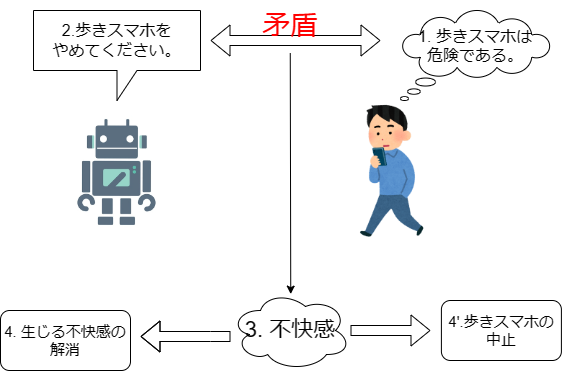
\includegraphics[width=13cm]{img/CDT.png}
  \caption{不快感が生じるまでの流れ}
\end{figure}

多くの人が歩きスマホのことを危険だと考えられており、さらに注意された際に不快感が生じることは示されている\cite{Schneider2022}。
具体的に、不快感が生じるまでの流れとして、図\ref{fig: dissonance}のように、(1)歩きスマホをしている人も信念として、歩きスマホが危険であると考えている。
(2)ロボットが注意を行う。(3)自分の行動と信念とが矛盾していることに気付かされ不快感が生じる。
(4)歩きスマホをやめる。(4')行動を変える以外の解消方法を行う。ここで、(4)ではなく(4')の行動を行った人を相手に対して、
有効な注意文言を考える。

\subsection{考えられる不快感の解消方法と有効な注意文言}
前節\ref{sec: dissonance}で述べたように、歩きスマホをしている人が注意された際に不快感が生じる。
\begin{table}[h]
  \centering
  \caption{歩きスマホによる不快感}
  \label{fig: UsingPhone}
  \begin{tabular}{c|c}
      認知1 & 歩きスマホは危険である  \\ \hline
      認知2 & 私は歩きスマホをしている \\
  \end{tabular}
\end{table}
この不快感は、図\ref{fig: UsingPhone}の、認知1と認知2が矛盾しているために生じるものである。
\ref{sec: CDT}章で述べたように、不快感を解消するために、いくつかの選択肢をとることができる。これらの選択肢の内、
1.行動を変えるという選択肢をとらせることが目的である。そのために、それ以外の選択肢をとった際に、その解消方法を無効にするような文言や、
新たに不快感を生じさせるような文言によって、再度不快感を解消する必要性を生み、1.行動を変えるという選択肢をとらせることが可能になると考える。

\subsubsection{行動を変える}
行動を変えることは、歩きスマホをやめることであり、この場合これ以上注意を行う必要はない。
\subsubsection{認知を変える}
認知を変えることは、表\ref{fig: UsingPhone}の認知1を「歩きスマホは危険ではない」とすることである。
この場合、注意文言として「歩きスマホによる死亡事故例も存在します」や「歩きスマホによって他人をケガさせた場合、高額の賠償金を請求される可能性があります」などが挙げられる。
\begin{table}[h]
  \centering
  \caption{認知の変更}
  \label{fig: AvoidDissonanceRevise}
  \begin{tabular}{c|c}
      認知1' & 歩きスマホは危険\sout{である}ではない \\ \hline
      認知2 & 私は歩きスマホをしている \\ \hline
      認知3 & 歩きスマホによる死亡事故が存在する \\\hline
  \end{tabular}
\end{table}
そのような注意を受けた場合、表\ref{fig: AvoidDissonanceRevise}のように、認知3が追加されることとなる。
そのような場合、認知1'と新たに追加された認知3の矛盾により新たに不快感が生じることとなる。
もしくは、認知1の変更が困難になる。それらの結果として、この方法での不快感の解消が難しく、再び不快感の解消を試みなければならない。
\subsubsection{新たな認知の追加}
不快感の解消のために、表\ref{fig: AvoidDissonance}の認知3や認知4が追加されることが考えられる。これらの認知は、
認知1と認知2の矛盾を軽減させることができるため、不快感の解消につながる。
\begin{table}[h]
  \centering
  \caption{新たな認知の追加}
  \label{fig: AvoidDissonance}
  \begin{tabular}{c|c}
      認知1 & 歩きスマホは危険である \\ \hline
      認知2 & 私は歩きスマホをしている \\ \hline
      認知3 & 地図アプリを見ており、これは必要な行為である \\\hline
      認知4 & 周りに人がおらず、他人に迷惑をかけていない \\ \hline
  \end{tabular}
\end{table}

そこで、これらの認知の追加に対しては、認知3の追加に対して「道案内なら私がしますよ。」や認知4の追加に対して
「そこの柱の裏から急に人が飛び出してくるかもしれません」といった文言が有効であると考えられる。
\begin{table}[h]
  \centering
  \caption{新たな認知の追加}
  \label{fig: AvoidDissonanceBlock}
  \begin{tabular}{c|c}
      認知1 & 歩きスマホは危険である \\ \hline
      認知2 & 私は歩きスマホをしている \\ \hline
      認知3 & 地図アプリを見ており、これは必要な行為である \\
      認知3' & 道案内を目の前の人に頼むことができる \\ \hline
      認知4 & 周りに人がおらず、他人に迷惑をかけていない \\ 
      認知4' & そこの柱の裏から急に人が飛び出してくるかもしれない \\ \hline
  \end{tabular}
\end{table}
なぜならば、これらの
文言は追加される認知と矛盾するものであり、図\ref{fig: AvoidDissonanceBlock}のように、認知3と認知3'の矛盾を生じさせることで、
新たな不快感が生まれる、もしくは、認知3の追加を防ぐことができると予想され、結果として、再び不快感の解消を試みなければならない。
そのためには、追加された認知を識別する必要があるが、これは人間のオペレータが存在することによって、
ある程度可能であることを前提としている。\footnote[1]{例えば、場所を探していそうならば、認知3の追加であるだろうし、周りに人がいないならば、認知4が追加される可能性が高い。}

\subsubsection{矛盾の矮小化、無視}
ロボットが矮小化や無視の対象となることが多い\cite{Schneider2022}。しかしながら、本研究ではアバターロボットを用い、肉声で注意を行うために、
この選択肢は選ばれづらいものと考え、この選択肢に対する注意文言は考えない。

\subsection{}
\section{移動操作の簡単化}
\subsection{---}
\subsection{---}

\chapter{評価実験}
\section{実験方法}
\section{実験結果}
\section{考察}

\chapter{まとめ}
研究のまとめ。なんやかんやなんやかんやなんやかんやなんやかんやなんやかんやなんやかんやなんやかんやなんやかんやなんやかんやなんやかんやなんやかんやなんやかんやなんやかんやなんやかんやなんやかんやなんやかんやなんやかんやなんやかんやなんやかんやなんやかんや

%=====================================================================================
\chapter*{謝辞} %章を付けずにタイトル表示
\addcontentsline{toc}{chapter}{謝辞} %章立てせずに目次に追加するおまじない
本論文を作成するにあたり、---- みなさまに感謝の意を表します.

%=====================================================================================

\addcontentsline{toc}{chapter}{参考文献} %章立てせずに目次に追加するおまじない
\renewcommand{\bibname}{参考文献} %これがないと,タイトルが「関連図書」になってしまう
\bibliography{citation.bib} %bibtexファイルの読み込み
\bibliographystyle{junsrt} %本文に\cite{}を入れることで,参考文献表示

\end{document}